\documentclass{beamer}

\pdfmapfile{+sansmathaccent.map}


\mode<presentation>
{
  \usetheme{Warsaw} % or try Darmstadt, Madrid, Warsaw, Rochester, CambridgeUS, ...
  \usecolortheme{seahorse} % or try seahorse, beaver, crane, wolverine, ...
  \usefonttheme{serif}  % or try serif, structurebold, ...
  \setbeamertemplate{navigation symbols}{}
  \setbeamertemplate{caption}[numbered]
} 


%%%%%%%%%%%%%%%%%%%%%%%%%%%%
% itemize settings

\definecolor{mypink}{RGB}{255, 30, 80}
\definecolor{mydarkblue}{RGB}{60, 160, 255}
\definecolor{myblue}{RGB}{240, 240, 255}
\definecolor{mygreen}{RGB}{0, 200, 0}
\definecolor{mygreen2}{RGB}{245, 255, 230}
\definecolor{mygray}{gray}{0.8}

\setbeamertemplate{itemize items}[default]

\setbeamertemplate{itemize item}{\color{mygreen}$\blacksquare$}
\setbeamertemplate{itemize subitem}{\color{mydarkblue}$\blacktriangleright$}
\setbeamertemplate{itemize subsubitem}{\color{mygray}$\blacksquare$}



\setbeamercolor{palette quaternary}{fg=white,bg=mydarkblue}
\setbeamercolor{titlelike}{parent=palette quaternary}

\setbeamercolor{palette quaternary2}{fg=black,bg=myblue}
\setbeamercolor{frametitle}{parent=palette quaternary2}



\setbeamerfont{frametitle}{size=\Large,series=\scshape}
\setbeamerfont{framesubtitle}{size=\normalsize,series=\upshape}





%%%%%%%%%%%%%%%%%%%%%%%%%%%%
% block settings

\setbeamercolor{block title}{bg=red!30,fg=black}

\setbeamercolor*{block title example}{bg=mygreen!40!white,fg=black}

\setbeamercolor*{block body example}{fg= black,
bg= mygreen2}


%%%%%%%%%%%%%%%%%%%%%%%%%%%%
% URL settings
\hypersetup{
    colorlinks=false,
    linkcolor=blue,
    filecolor=blue,      
    urlcolor=blue,
}

%%%%%%%%%%%%%%%%%%%%%%%%%%

\renewcommand{\familydefault}{\rmdefault}

\usepackage{amsmath}
\usepackage{mathtools}


\usepackage{subcaption}

\newcommand{\bo}[1] {\mathbf{#1}}
\newcommand{\R} {\mathbb{R}}
\DeclareMathOperator*{\argmin}{arg\,min}


%%%%%%%%%%%%%%%%%%%%%%%%%%%%
% code settings

\usepackage{listings}
\usepackage{color}
% \definecolor{mygreen}{rgb}{0,0.6,0}
% \definecolor{mygray}{rgb}{0.5,0.5,0.5}
\definecolor{mymauve}{rgb}{0.58,0,0.82}
\lstset{ 
  backgroundcolor=\color{white},   % choose the background color; you must add \usepackage{color} or \usepackage{xcolor}; should come as last argument
  basicstyle=\footnotesize,        % the size of the fonts that are used for the code
  breakatwhitespace=false,         % sets if automatic breaks should only happen at whitespace
  breaklines=true,                 % sets automatic line breaking
  captionpos=b,                    % sets the caption-position to bottom
  commentstyle=\color{mygreen},    % comment style
  deletekeywords={...},            % if you want to delete keywords from the given language
  escapeinside={\%*}{*)},          % if you want to add LaTeX within your code
  extendedchars=true,              % lets you use non-ASCII characters; for 8-bits encodings only, does not work with UTF-8
  firstnumber=0000,                % start line enumeration with line 0000
  frame=single,	                   % adds a frame around the code
  keepspaces=true,                 % keeps spaces in text, useful for keeping indentation of code (possibly needs columns=flexible)
  keywordstyle=\color{blue},       % keyword style
  language=Octave,                 % the language of the code
  morekeywords={*,...},            % if you want to add more keywords to the set
  numbers=left,                    % where to put the line-numbers; possible values are (none, left, right)
  numbersep=5pt,                   % how far the line-numbers are from the code
  numberstyle=\tiny\color{mygray}, % the style that is used for the line-numbers
  rulecolor=\color{black},         % if not set, the frame-color may be changed on line-breaks within not-black text (e.g. comments (green here))
  showspaces=false,                % show spaces everywhere adding particular underscores; it overrides 'showstringspaces'
  showstringspaces=false,          % underline spaces within strings only
  showtabs=false,                  % show tabs within strings adding particular underscores
  stepnumber=2,                    % the step between two line-numbers. If it's 1, each line will be numbered
  stringstyle=\color{mymauve},     % string literal style
  tabsize=2,	                   % sets default tabsize to 2 spaces
  title=\lstname                   % show the filename of files included with \lstinputlisting; also try caption instead of title
}

%%%%%%%%%%%%%%%%%%%%%%%%%%%%
% tikz settings

\usepackage{tikz}
\tikzset{every picture/.style={line width=0.75pt}}

%%%%%%%%%%%%%%%%%%%%%%%%%%%%

\usepackage{qrcode}



\title{Laplace Transform and Transfer Functions}
\subtitle{Control Theory, Lecture 3}
\author{by Sergei Savin}
\centering
\date{\mydate}



\begin{document}
\maketitle


\begin{frame}{Content}

\begin{itemize}
\item ODE solutions
\item Laplace Transform
\item Laplace Transform of a derivative
\item Derivative operator
\item Transfer Function
    \begin{itemize}
    \item Example
    \item Interesting things done easy
    \end{itemize}
\item State-Space to Transfer Function conversion
\item Read more
\end{itemize}

\end{frame}





\begin{frame}{ODE solutions}
% \framesubtitle{O}
\begin{flushleft}

\begin{equation}
    \begin{bmatrix}
    \dot x_1 \\ \dot x_2 \\ \dot x_3
    \end{bmatrix}
    \begin{bmatrix}
    0 & 1 & 0 \\ 0 & 0 & 1 \\ -5 & -10 & -10
    \end{bmatrix}
    \begin{bmatrix}
    x_1 \\ x_2 \\ x_3
    \end{bmatrix}
    +
    \begin{bmatrix}
    0\\ 0 \\ 10
    \end{bmatrix}
    u
\end{equation}

\begin{figure}
\minipage{0.32\textwidth}
  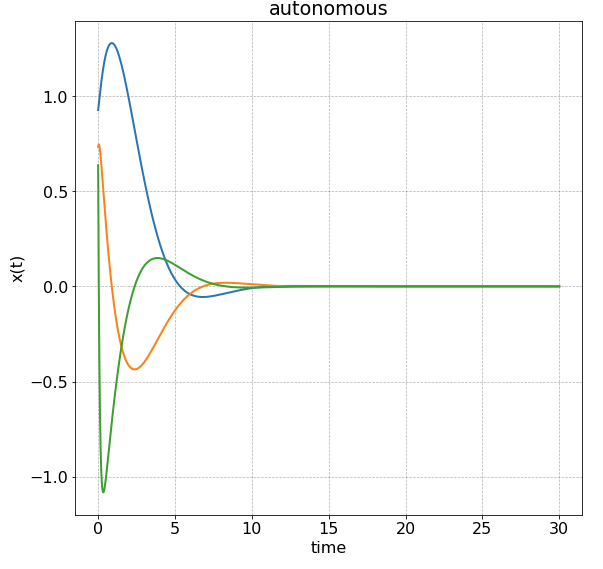
\includegraphics[width=\linewidth]{Autonomous.png}
\caption{Autonomous ODE ($u = 0$)}
\endminipage\hfill
\minipage{0.32\textwidth}
  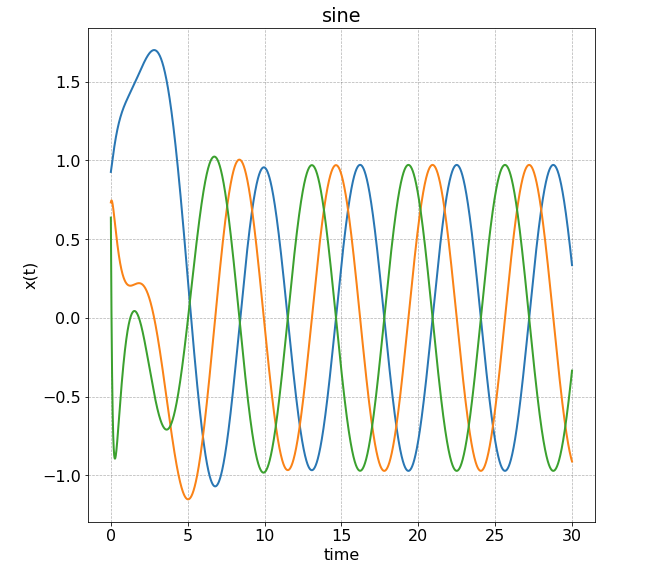
\includegraphics[width=\linewidth]{sine.png}
\caption{reaction to sine wave ($u = sin(t)$)}
\endminipage\hfill
\minipage{0.32\textwidth}%
  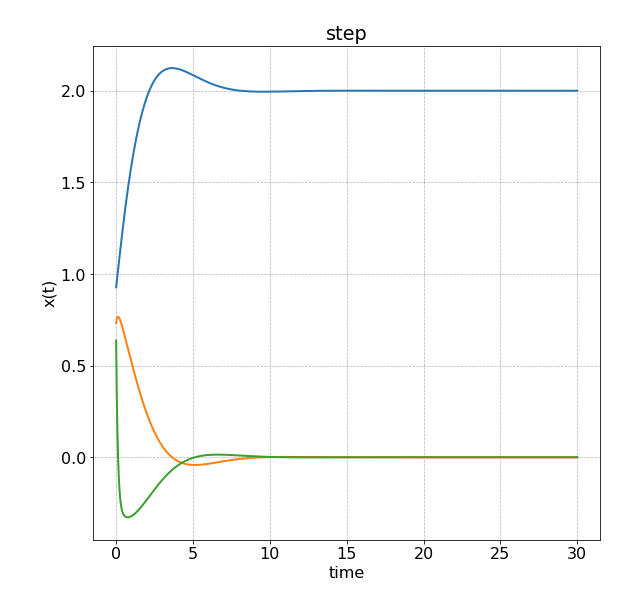
\includegraphics[width=\linewidth]{step.png}
\caption{Reaction to step function ($u = 1$)}
\endminipage
\end{figure}

\end{flushleft}
\end{frame}


\begin{frame}{Laplace Transform}
% \framesubtitle{O}
\begin{flushleft}

By definition, Laplace transform of a function $f(t)$ is given as:

\begin{equation}
    F(s) = \int_0^\infty f(t) e^{-st}dt
\end{equation}

where $F(s)$ is called an \emph{image} of the function.

\bigskip

The study of Laplace transform is a separate mathematical field with applications in solving ODEs, which we won't cover. However, we will consider transform of one case of interest - transform of a derivative. 

\end{flushleft}
\end{frame}



\begin{frame}{Laplace Transform of a derivative}
% \framesubtitle{O}
\begin{flushleft}

Consider a derivative $\frac{dx}{dt}$ and its transform:

\begin{equation}
    \mathcal{L}\left(\frac{dx}{dt}\right) = \int_0^\infty \frac{dx}{dt} e^{-st}dt
\end{equation}

we will make use of the integration by parts formula:

\begin{block}{Integration by parts}
\begin{equation}
\int v \frac{du}{dt} dt = vu - 
\int \frac{dv}{dt} u dt    
\end{equation}
\end{block}

In our case, $\frac{du}{dt} = \frac{dx}{dt}$, $u = x$, $v = e^{-st}$, $\frac{dv}{dt} = -se^{-st}$:

\begin{equation}
\mathcal{L}\left(\frac{dx}{dt}\right) = \left[x e^{-st} \right]_0^\infty - 
\int_0^\infty -se^{-st} x dt  
\end{equation}

\begin{equation}
\mathcal{L}\left(\frac{dx}{dt}\right) = -x(0) + s\mathcal{L}(x)  
\end{equation}

\end{flushleft}
\end{frame}




\begin{frame}{Derivative operator}
% \framesubtitle{O}
\begin{flushleft}

Thus, assuming that $x(0) = 0$, we can obtain a \emph{derivative operator}:

\begin{equation}
\label{eq:NoIC_laplace}
\mathcal{L}\left(\frac{dx}{dt}\right) = s \mathcal{L}\left(x\right)
\end{equation}

\bigskip

Please notice that \eqref{eq:NoIC_laplace} is only true when $x(0) = 0$; it generally does not look very elegant either. Introducing a big-time abuse of notation, we can denote $x(s) = \mathcal{L}\left(x\right)$ and then drop the brackets, leaving us with:

\begin{equation}
\frac{dx}{dt} \longrightarrow s x
\end{equation}

This form of a derivative operator has a very strange notation in terms of the Laplace transform theory, but is very simple to use in practice.

\end{flushleft}
\end{frame}



\begin{frame}{Transfer Function}
% \framesubtitle{O}
\begin{flushleft}

Consider the following ODE, where $u$ is an input (function of time that influences the solution of the ODE):

\begin{equation}
\ddot x + a \dot x + b x = u
\end{equation}

We can rewrite it using the derivative operator:

\begin{equation}
s^2 x + a s x + b x = u
\end{equation}

and then collect $x$ on the left-hand-side:

\begin{equation}
x = \frac{1}{s^2 + a s + b} u
\end{equation}

At this point the mathematical meaning of this expression as an ODE is very vague, but it has a different direct use; this form is called a \emph{transfer function}.

\end{flushleft}
\end{frame}


\begin{frame}{Transfer Function}
\framesubtitle{Examples}
\begin{flushleft}

\begin{example}
Given ODE: $2 \dddot x + 5\dot x - 40 x = 10 u$

The transfer function for it looks: 
$x = \frac{10}{2 s^3 + 5 s - 40} u$
\end{example}


\begin{example}
Given ODE: $2 \dot x - 4 x = u$

The transfer function for it looks: $x = \frac{1}{2 s - 4} u$
\end{example}


\begin{example}
Given ODE: $3 \dddot x + 4x = u$

The transfer function for it looks: $x = \frac{1}{2 s^3 + 4} u$
\end{example}

\end{flushleft}
\end{frame}




\begin{frame}{Transfer Function}
\framesubtitle{Interesting things done easy}
\begin{flushleft}

Consider the following (strange) ODE:

\begin{equation}
2 \ddot x + 3 \dot x + 2 x = 10 \dot u - u
\end{equation}

Using the differential equation:

\begin{equation}
2 s^2 x + 3s x + 2x = 10s u - u
\end{equation}

...which is the same as:

\begin{equation}
(2s^2 + 3s + 2)x = (10s - 1)u
\end{equation}

The transfer function for it looks: 

\begin{equation}
x = \frac{10s - 1}{2s^2 + 3s + 2} u
\end{equation}

\end{flushleft}
\end{frame}




\begin{frame}{State-Space to Transfer Function conversion}
% \framesubtitle{O}
\begin{flushleft}

Transfer functions are being used to study the relation between the input and the output of the dynamical system.

\bigskip

Consider standard form state-space dynamical system:

\begin{equation}
\begin{cases}
\dot{\bo{x}} = \bo{A}\bo{x} + \bo{B}\bo{u} \\
     \bo{y}  = \bo{C}\bo{x} + \bo{D}\bo{u}
\end{cases}
\end{equation}

We can rewrite it using the derivative operator:

\begin{equation}
\begin{cases}
s\bo{I}\bo{x} -\bo{A}\bo{x} = \bo{B}\bo{u} \\
\bo{y}  = \bo{C}\bo{x} + \bo{D}\bo{u}
\end{cases}
\end{equation}

and then collect $\bo{x}$ on the left-hand-side: $\bo{x} = (s\bo{I} -\bo{A})^{-1} \bo{B}\bo{u}$

and finally, express $\bo{y}$ out:

\begin{equation}
\bo{y}  = \left( \bo{C}(s\bo{I} -\bo{A})^{-1} \bo{B} + \bo{D} \right) \bo{u}
\end{equation}

\end{flushleft}
\end{frame}



\begin{frame}{Transfer Function and Control (0)}
	% \framesubtitle{O}
	\begin{flushleft}
		
		Let the dynamic system be described as a transfer function:
		
		\begin{equation}
			y = G(s) x
		\end{equation}
		
		We can try to modify the input based on how the output looks-like. Since we always do it in a linear way, we can write it as:
		
		\begin{equation}
			y = G(s) (x - H(s) y)
		\end{equation}
		
		where $H(s) y$ is called \emph{feedback}.
		
		\bigskip
		
		How would the transfer function from $x$ to $y$ look like? 
		
	\end{flushleft}
\end{frame}


\begin{frame}{Transfer Function and Control (1)}
	% \framesubtitle{O}
	\begin{flushleft}
		
		From $y = G(s) (x - H(s) y)$ we go:
		
		\begin{equation}
			y = G(s)x - G(s)H(s) y
		\end{equation}
		\begin{equation}
			y + G(s)H(s) y = G(s)x
		\end{equation}
		\begin{equation}
			y = \frac{G(s)}{1 + G(s)H(s)} x
		\end{equation}
		
		Thus, we found \emph{closed-loop} transfer function:
		
		\begin{equation}
			W(s) = \frac{G(s)}{1 + G(s)H(s)}
		\end{equation}
		
	\end{flushleft}
\end{frame}



\begin{frame}{Read more}

\begin{itemize}
\item \bref{https://www.cds.caltech.edu/~murray/courses/cds101/fa04/caltech/am04_ch6-3nov04.pdf}{Chapter 6 Transfer Functions}

\item \bref{https://youtu.be/RJleGwXorUk}{Control Systems Lectures - Transfer Functions, by Brian Douglas}

\item \bref{https://youtu.be/ZGPtPkTft8g}{The Laplace Transform - A Graphical Approach, by Brian Douglas}

\end{itemize}

\end{frame}



\begin{frame}{Thank you!}
\centerline{Lecture slides are available via Moodle.}
\bigskip
\centerline{You can help improve these slides at:}
\centerline{\mygit}
\bigskip
\centerline{Check Moodle for additional links, videos, textbook suggestions.}
\bigskip

\centerline{\textcolor{black}{\qrcode[height=1.6in]{https://github.com/SergeiSa/Control-Theory-Slides-Spring-2022}}}
\end{frame}

\end{document}
